\documentclass{article}

\usepackage{amssymb}
\usepackage{pgf}
\usepackage{tikz}
\usetikzlibrary{arrows,automata}
\usepackage[latin1]{inputenc}

\title{Project 2}
\author{Jesse Adams, Dominic Orsi, Ben Puryear}
\date{September 14th, 2023}

\begin{document}

\maketitle

Let an FSA, $M$ be defined as follows:

$Q = \{q_1, q_2, q_3\}$

$\Sigma = {0,1}$

$F = {q_2}$

$q_s = q_1$


$\delta = $
\begin{tabular}{ |c|c|c| }
          & 0     & 1     \\
    \hline
    $q_1$ & $q_1$ & $q_2$ \\
    $q_2$ & $q_3$ & $q_2$ \\
    $q_3$ & $q_2$ & $q_2$ \\
\end{tabular}


\section{Draw $M$ using nodes and arcs.}
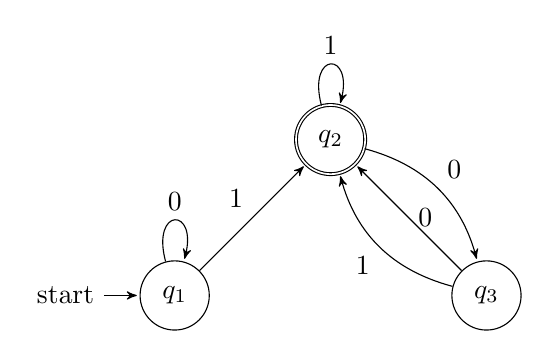
\begin{tikzpicture}[->,>=stealth',shorten >=1pt,auto,node distance=2.8cm]
    \tikzstyle{every state}=[fill=none,draw=black,text=black]
    \node[initial,state]  (1)                     {$q_1$};
    \node[state, double]  (2) [above right of=1]  {$q_2$};
    \node[state]          (3) [below right of=2]  {$q_3$};
    \path (1) edge [loop above]   node            {0} (1)
    edge                node            {1} (2)
    (2) edge [bend left]    node            {0} (3)
    edge [loop above]   node            {1} (2)
    (3) edge                node [right]    {0} (2)
    edge [bend left]    node            {1} (2);
\end{tikzpicture}

\section{Characterize $L(M)$ in words, the more formal the better.}

The language $L(M)$ can be characterized as any string built from the characters $\{0, 1\}$ containing at least one $1$, and ending with either a $1$ or an even number of $0$s. \\
% $L(M)\{s|1 \in s$ followed by an even number of $0$s$\}$
$L(M)\{s$ ends with a $1$ or $00\}$
\newpage

The formal description of a DFA $M_1$ is:

$Q = \{q_1, q_2,q_3,q_4,q_5\}$

$\Sigma = \{u,d\}$

$\delta$: is described in the table below

$q_s = q_3$

$F = \{q_3\}$
\begin{center}
    Here is $\delta$:
    \begin{tabular}{ |c|c|c| }
              & $u$   & $d$   \\
        \hline
        $q_1$ & $q_1$ & $q_2$ \\
        $q_2$ & $q_1$ & $q_3$ \\
        $q_3$ & $q_2$ & $q_4$ \\
        $q_4$ & $q_3$ & $q_5$ \\
        $q_5$ & $q_4$ & $q_5$ \\
    \end{tabular}
\end{center}

\section{Why is $F$ a set, whereas $q_s$ is not?}

$F$ is a set because it is all the accept states where as $q_s$ is the start state and in an FSA there is only one start stat but there can be multiple accept states.

\section{Give the state diagram of $M_1$}

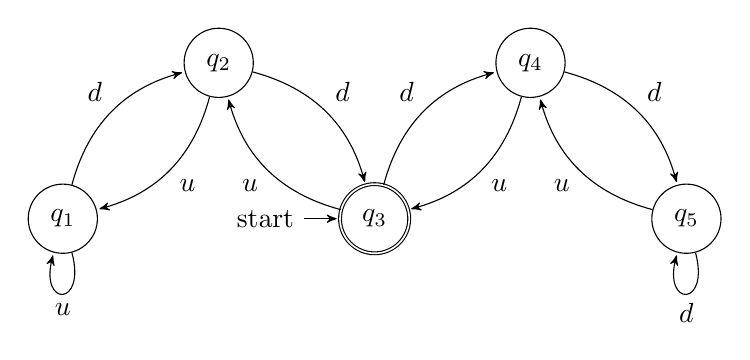
\begin{tikzpicture}[->,>=stealth',shorten >=1pt,auto,node distance=2.8cm]
    \tikzstyle{every state}=[fill=none,draw=black,text=black]
    \node[state]                  (1)                     {$q_1$};
    \node[state]                  (2) [above right of=1]  {$q_2$};
    \node[initial, state, double] (3) [below right of=2]  {$q_3$};
    \node[state]                  (4) [above right of=3]  {$q_4$};
    \node[state]                  (5) [below right of=4]  {$q_5$};
    \path (1) edge [loop below]   node {$u$} (1)
    edge [bend left]    node {$d$} (2)
    (2) edge [bend left]    node {$u$} (1)
    edge [bend left]    node {$d$} (3)
    (3) edge [bend left]    node {$u$} (2)
    edge [bend left]    node {$d$} (4)
    (4) edge [bend left]    node {$u$} (3)
    edge [bend left]    node {$d$} (5)
    (5) edge [bend left]    node {$u$} (4)
    edge [loop below]   node {$d$} (5);
\end{tikzpicture}


\section{Suppose we have a machine, $M_2$, an DFA, whose alphabet is $\{a,b\}$. Suppose further that $L(M_2) = \{w|w$ has an odd number of the symbol a and ends with the symbol b$\}$. Give the state diagram of $M_2$}

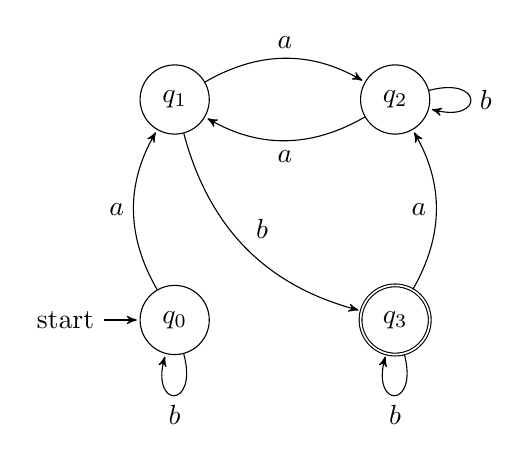
\begin{tikzpicture}[->,>=stealth',shorten >=1pt,auto,node distance=2.8cm]
    \tikzstyle{every state}=[fill=none,draw=black,text=black]
    \node[initial,state]  (1)                     {$q_0$};
    \node[state]          (2) [above of=1]        {$q_1$};
    \node[state]          (3) [right of=2]        {$q_2$};
    \node[state, double]  (4) [below of=3]        {$q_3$};
    \path (1) edge [loop below]   node {$b$} (1)
    edge [bend left]    node {$a$} (2)
    (2) edge [bend right]   node {$b$} (4)
    edge [bend left]    node {$a$} (3)
    (3) edge [bend left]    node {$a$} (2)
    edge [loop right]   node {$b$} (3)
    (4) edge [bend right]   node {$a$} (3)
    edge [loop below]   node {$b$} (4);
\end{tikzpicture}

\section{Suppose we have a machine, $M_3$, a DFA, whose alphabet is $\{a,b\}$. Suppose further that $L(M_3) = \{w|w$ is not in $a^*b^*\}$. $L(M_3)$ is the complement of a simpler language. Construct the DFA for the simpler language, then use it to give the state diagram of $L(M_3)$.}

$M_3 : \Sigma = {a,b}$ \\
$L(M_3) = \{w | w$ is not in $a^* b^*\}$ \\
$L(M_{3_0}) = \{w | w$ is in $a^* b^*\} \rightarrow \{a, b, ab, abb, aabb, ...\}$

\begin{center}
    $M_3$\\
    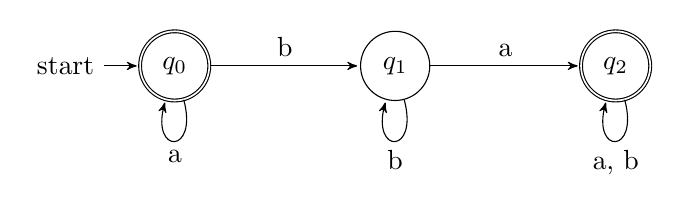
\begin{tikzpicture}[->,>=stealth',shorten >=1pt,auto,node distance=2.8cm]
        \tikzstyle{every state}=[fill=none,draw=black,text=black]
        \node[initial,state, double]    (1)                 {$q_0$};
        \node[state ]                   (2) [right of=1]    {$q_1$};
        \node[state, double]            (3) [right of=2]    {$q_2$};
        \path   (1) edge [loop below]   node {a}    (1)
        edge []             node {b}    (2)
        (2) edge []             node {a}    (3)
        edge [loop below]   node {b}    (2)
        (3) edge [loop below]   node {a, b} (3);
    \end{tikzpicture}
\end{center}

\section{Suppose we have a machine, $M_4$, a DFA, whose alphabet is $\{0,1\}$.  Suppose further that  $L(M_4) = \{w|w$ contains an even number of 0s or contains exactly two 1s$\}$. Give the state diagram for $M_4$}

$M_4 : \Sigma = \{0,1\}$\\
$L(M_4) = \{w | w$ contains even \# of $0$s of exactly 2 $1$s $\}$\\
$\{w | w$ contains even \# of $0$s of exactly 2 $1$s $\} = \{00,11,00011,0110,11001,...\}$

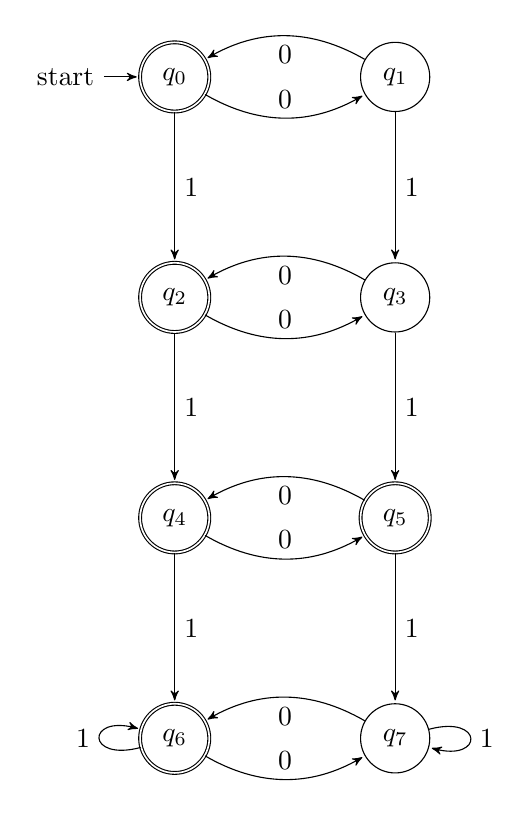
\begin{tikzpicture}[->,>=stealth',shorten >=1pt,auto,node distance=2.8cm]
    \tikzstyle{every state}=[fill=none,draw=black,text=black]
    \node[initial,state, double]  (1)                     {$q_0$};
    \node[state]                  (2) [right of=1]        {$q_1$};
    \node[state,double]           (3) [below of=1]        {$q_2$};
    \node[state]                  (4) [right of=3]        {$q_3$};
    \node[state,double]           (5) [below of=3]        {$q_4$};
    \node[state,double]           (6) [right of=5]        {$q_5$};
    \node[state,double]           (7) [below of=5]        {$q_6$};
    \node[state]                  (8) [right of=7]        {$q_7$};
    \path (1) edge []             node {1} (3)
    edge [bend right]   node {0} (2)
    (2) edge []             node {1} (4)
    edge [bend right]   node {0} (1)
    (3) edge []             node {1} (5)
    edge [bend right]   node {0} (4)
    (4) edge []             node {1} (6)
    edge [bend right]   node {0} (3)
    (5) edge []             node {1} (7)
    edge [bend right]   node {0} (6)
    (6) edge []             node {1} (8)
    edge [bend right]   node {0} (5)
    (7) edge [bend right]   node {0} (8)
    edge [loop left]    node {1} (7)
    (8) edge [bend right]   node {0} (7)
    edge [loop right]   node {1} (8);
\end{tikzpicture}

\end{document}